%%%%%%%%%%%%%%%%%%%%%%%%%%%%%%%%
% INCLUSION PREAMBULE COMMUN   %
%%%%%%%%%%%%%%%%%%%%%%%%%%%%%%%%
% définition et packages du présent fichier
%%%%%%%%%%%%%%%%%%%%%%%%%
% PACKAGES              %
%%%%%%%%%%%%%%%%%%%%%%%%%
\documentclass{report}
\usepackage[utf8x]{inputenc}  % accents
\usepackage{geometry}         % marges
\usepackage[francais]{babel}  % langue
\usepackage{graphicx}         % images
\usepackage{verbatim}         % texte préformaté
\usepackage{fancyhdr}         % fancy






% Titre de ce fichier dans le fancy 
\newcommand{\titre}{{\Huge Cahier des charges}\\Groupe B}
\newcommand{\titrehead}{Cahier des charges}
% Inclusion du préambule commun
%%%%%%%%%%%%%%%%%%%%%%%%%
% PRÉAMBULE             %
%%%%%%%%%%%%%%%%%%%%%%%%%
\title{\titre{}}
\author{}
% laisser vide pour date de compilation
\date{} 

% FORMAT PAGES         
\pagestyle{fancy} % nom du rendu (définit les lignes suivantes)
        \lhead{} % left head
        \chead{\titrehead{}} % center head
        \rhead{} % right head
        \lfoot{} % left foot
        \cfoot{\thepage} % center foot
        \rfoot{} % right foot


% Ce fichier est un préambule commun à toutes les sources LaTeX.
% Il est inclus par toutes les sources et permet d'avoir un formatage commun facilement modifiable.


%

%%%%%%%%%%%%%%%%%%%%%%%%%
% BEGIN                 %
%%%%%%%%%%%%%%%%%%%%%%%%%
\begin{document}
\maketitle
\tableofcontents



%%%%%%%%%%%%%%%%%%%%%
% CHAPTER 1         %
%%%%%%%%%%%%%%%%%%%%%
\chapter{Présentation du projet}


\section{Contexte}
        \paragraph*{}
        Le présent cahier des charges correspond au projet du second semestre de Licence 3 de Spi, un Picross.\\
        Sont ici dressées les exigences, les besoins du client et les fontionnalités qui seront présentes dans le jeu.


\section{Objectif}
        \paragraph*{}
        L'objectif est l'étude et la réalisation d'un Picross. Ainsi, le jeu devra pouvoir proposer plusieurs services aux joueurs :
        \begin{itemize}
                \item le choix d'une grille parmi plusieurs possibilités de taille;
                \item utilisation d'une aide au jeu;
                \item possibilité de sauvegarder et de charger une grille en cours de résolution;
                \item consulter les scores et classements;
                \item éditer sa propre grille et la sauvegarder pour l'ajouter à la liste des grilles jouables.
        \end{itemize}


\section{Description de l'existant}
        \paragraph*{}
        \begin{itemize}
                \item de nombreuses applications proposent des jeux de Picross ou équivalents, notamment sur le web où il est possible de trouver de nombreuses grilles et variantes;
                \item le présent projet s'appuiera sur des algorithmes déjà définis pour les traitements d'aide;
                \item des modules connus et reconnus seront utilisés pour des opérations de base telles que la sérialisation;
                \item des sources internet telles que wikipédia sont utilisées pour fixer les définitions propres au Picross.
        \end{itemize}


\section{Critères d'acceptabilité du produit}
        \paragraph*{}
        L'application doit répondre aux critères suivants :
        \begin{itemize}
          \item validation des objectifs demandés par le client;
                \item validation du produit via un dossier de tests réalisés par notre groupe;
                \item respect des choix technologiques du client (cf. \textit{contraintes techniques});
                \item jeu picross;
                \item chronomètre pour la mesure du temps de jeu;
                \item interface graphique GTK;
                \item aide à l'utilisateur pour la résolution du jeu.
        \end{itemize}




%%%%%%%%%%%%%%%%%%%%%
% CHAPTER 2         %
%%%%%%%%%%%%%%%%%%%%%
\chapter{Analyse des besoins} 


\section{Liste des acteurs}
        \paragraph*{}
        L'utilisateur qui jouera au Picross constituera le seul acteur du logiciel.


\section{Expression des besoins}
        \paragraph*{}
        Le client demande la réalisation d'un jeu de Picross proposant certains services décrits dans les fonctionnalités. 

        %\paragraph*{} % redondant avec la première phrase
        %Le client souhaiterait également l'ajout d'une aide afin de permettre aux joueurs de se débloquer si besoin.


\section{Besoins fonctionnels}
        \paragraph*{}
        L'utilisateur devra pouvoir jouer une partie de picross dans la barre de menu. Cela ouvrira une fenêtre où il pourra choisir la taille du jeu  parmi des valeurs prédéfinies (5*5, 10*10, 15*15, 20*20, 25*25). 
        \paragraph*{}
        Il pourra demander de l'aide au programme qui donnera une indication ou effectuera une modification du jeu selon la volonté de l'utilisateur.
        \paragraph*{}
        Il pourra aussi éditer une grille à la main ou/et à partir d'une image.
        \paragraph*{}
        Il pourra enfin sauvegarder sa partie, la charger, et consulter les statistiques des victoires de tous les joueurs (ou seulement les siennes) sur la grille courante.


%\section{Besoins non-fonctionnels} % Pour le moment, ce n'est pas nécessaire.
        %\paragraph*{}
        %Calculs statistiques relatives à chaque grille.
        %\paragraph*{}
        %Modules de sérialisation, 


\section{Fonctionnalités}
        \paragraph*{}
        \begin{tabular*}{0.75\textwidth}{ c | c }
                Référence & Fonctionnalité\\
                & Programme \\ 
                F01 & Quitter le programme \\
                F02 & Consulter les informations complémentaires du programme \\
                F03 & Afficher des informations relatives à la grille et à l'aide \\
                & Jeu \\ 
                F11 & Modifier la grille de jeu par un clic de souris \\
                F12 & Consulter le timer du jeu \\
                F13 & Consulter le meilleur score sur la grille courante \\
                F14 & Utiliser l'aide \\
                F15 & Utiliser l'aide avancée \\
                & Données \\ 
                F21 & Sauvegarder une grille \\
                F22 & Charger une grille \\
                F23 & Créer une nouvelle grille \\ % NB : au lancement du jeu : une au hasard parmi celles existantes.
        \end{tabular*}

        \paragraph*{}
        Details des fonctionnalités.
        \begin{description}
                \item[F01 :] appuyer sur un bouton permet de quitter le jeu et demande à l'utilisateur s'il veut sauvegarder avant de quitter
                \item[F02 :] un bouton permet l'affichage d'une pop-up contenant des informations concernant le programme (modules et bibliothèques, licences,...)
                \item[F03 :] une zone de texte dans l'interface principale communiquant des informations à l'utilisateur (notamment en relation avec l'aide)
                \item[F11 :] modification de l'état d'une case de la grille à l'aide d'un clic de souris, et modification par bande: lorsque le curseur est enfoncé, tant qu'il n'est pas relaché, toutes les cases par lesquelles on est passé deviennent noires, ou croisées(c'est selon)\\
                \item[F12 :] indication du temps passé sur la grille courante
                \item[F13 :] indication du temps de résolution et du nombre d'appels à l'aide pour le meilleur score de la grille courante
                \item[F14 :] afficher une indication visuelle sur une colonne ou une ligne facilement résolvable avec explication textuelle de la technique utilisée
                \item[F15 :] afficher une indication visuelle sur une colonne ou une ligne, où le programme indiquera explicitement quelles cases modifier
                \item[F21 :] sauvegarder la grille en cours de résolution avec en nom par défaut, la taille de la grille ainsi que sa date de sauvegarde
                \item[F22 :] charger une grille précédemment sauvegardée
                \item[F23 :] créer une nouvelle grille  à partir d'une grille que l'utilisateur aura lui-même dessinée à l'aide  de l'interface graphique du programme, ou depuis une image; cette grille aura par défaut la même taille que la précédente grille jouée
        \end{description}


\section{Scénario d'utilisation}
        \paragraph*{}
        Lorsque l'application est démarrée, une grille de la taille de la grille précédente est générée depuis les grilles connues du programme, et le timer est mis en marche. L'utilisateur peut donc, jouer cette grille, générer une autre grille, ou charger une partie précédemment sauvegardée.
        \paragraph*{}
        Pour éditer une nouvelle grille, l'utilisateur cliquera sur le bouton \textit{éditer} qui ouvrira la fenêtre d'édition de grille.
        Cette fenêtre permettra à l'utilisateur d'annuler l'édition, de valider sa grille, d'importer une image, de donner un nom à la grille et de modifier la grille et sa taille.\\
        Importer une image modifie l'ensemble de la grille.
        Lorsque l'utilisateur valide sa grille, elle est sauvegardée dans la liste des grilles du programme, et lui est immédiatement proposée comme grille à résoudre après que la fenêtre d'édition de grille ait été fermée.\\
        \paragraph*{}
        Pour charger une grille en cours de résolution, une fenêtre s'ouvre, montrant alors l'ensemble des parties enregistrées. L'utilisateur choisira alors celle qu'il désirera continuer.
        \paragraph*{}
        Lorsque l'utilisateur sauvegarde le jeu en cours avec comme nom par défaut :la taille de la grille ainsi que sa date. Ce nom permettra d'identifier la sauvegarde lors du chargement futur de la partie.


        %\section{Diagramme de classe} # NON ATTENDU DANS LE CAHIER DES CHARGES, PLUTÔT DANS LE CAHIER DE CONCEPTION
        %\paragraph*{}
        %Afin de mettre au clair l'architecture de l'application, un diagramme de classe est définit : 
        %\begin{center}
                %\includegraphics[scale=1]{data/classDiagram.png}\\
                %\textbf{Diagramme de Classe UML}
        %\end{center}


%%%%%%%%%%%%%%%%%%%%%%
% CHAPTER 3          %
%%%%%%%%%%%%%%%%%%%%%%
\chapter{Contraintes}


\section{Documentation}
        \paragraph*{}
        \begin{description}
                \item[Cahier des charges :] spécifier les besoins du client, les fonctionnalités attendues de l’application, ainsi que les contraintes et les livrables du projet;
                \item[dossier de spécification :] présenter la conception des différents modules que comportera l’application;
                \item[dossier de tests :] montrer toutes les procédures de test, les résultats attendus ainsi que les résultats obtenus;
                \item[procédure d'installation:] expliquer à l’utilisateur comment installer et utiliser cette application;
                \item[rapport de projet:] résumer ce qui a été fait lors du projet, les difficultés rencontrées.
        \end{description}


\section{Contraintes techniques}
        \paragraph*{}
        \begin{itemize}
                \item Le système est principalement conçu pour fonctionner sous architecture UNIX;% mais aussi compatible avec le système Windows. % euh, attention, les fichiers nécessiteront peut-être un traitement particulier sous windows
                \item ruby est utilisé comme langage principal;
        \end{itemize}


%%%%%%%%%%%%%%%%%%%%
% CHAPTER 4        %
%%%%%%%%%%%%%%%%%%%%
\chapter{Déroulement du projet}


\section {Livrables}
        \paragraph*{}
        Les documents suivants seront livrés sous forme électronique et feront l'objet d'une validation par le client :
        \begin{itemize}
                \item le présent cahier des charges validé par le client;
                \item les cahiers d'analyse et de conception;
                \item le code source;
                \item le logiciel qui respecte le cahier des charges;
                \item un manuel utilisateur, explicitant le principe du jeu, détaillant les techniques, et expliquant l'interface du programme.
        \end{itemize}


\section{Contraintes temporelles}
        \paragraph*{}
        Afin de mener à bien ce projet , il est mis à disposition des étudiants 16 séances de 3h pour permettre aux membres de l'équipe d'établir les points importants sur lesquels travailler.
        \paragraph*{}
        La période de développement de l’application s’étend du 24 janvier au 16 Mai 2014 suivi d’une présentation finale de l’application. % dates à vérifier
        \paragraph*{}
        Le jeu devra être rendu le \textbf{16 mai 2014}, ainsi que tous les livrables qui composent le projet.
        Le planning prévisionnel est traduit en diagramme de Gantt :\\

        \begin{center}
                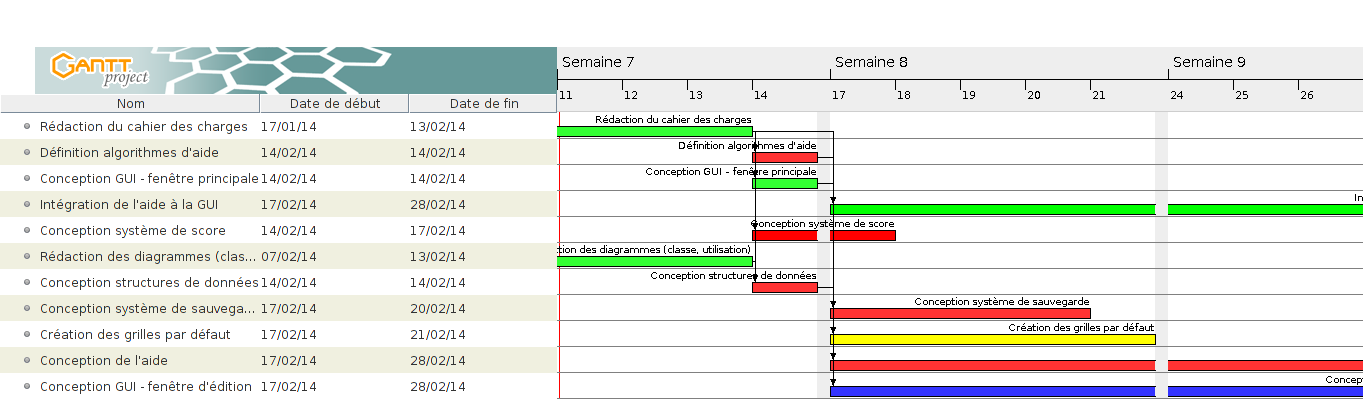
\includegraphics[scale=.6, angle=90]{data/ganttDiagram.png}\\
                \textbf{Diagramme de Gantt prévisionnel}
        \end{center}


\section {Equipe}
        \paragraph*{}
        Les membres de l'équipe sont 
        \begin{itemize}
                \item Charlie Maréchal (documentaliste);
                \item Ewen Cousin (développeur);
                \item Jaweed Parwany (développeur);
                \item Julien Le Gall (développeur);
                \item Lucas Bourneuf (chef d'équipe);
                \item Nicolas Bourdin(développeur);
        \end{itemize}


\section{Outils de développement}
        \paragraph*{}
        \begin{enumerate}
                \item irb pour l'interprétation du code Ruby 1.9;
                \item Ruby-GTK pour le développement de l'interface graphique;
                %\item le jeu doit supporter plusieurs langues(pas obligatoire pour l'instant); % Absolument pas demandé; le zonage dépend de la GUI.
                \item YAML pour la gestion des sauvegardes; % yaml est plus rapide. L'intérêt de marshall est de rendre les data lisibles, ce qui n'est pas attendu.
                \item rmagick pour la génération de grille depuis les images de l'utilisateur;
                \item glib pour le chronométrage;
                \item rdoc pour la génération de documentation de code.
        \end{enumerate}


\end{document}
% END
